%!TEX root = ../../diachron-D5_2.tex

\subsection{The Dataset Quality Ontology}
\label{sec:DAQ} 
% describe the ontology which is used to describe the quality metadata of a dataset
The idea behind the Dataset Quality Ontology~\cite{DebattistaEtAl:daQ:LDOW:2014}\footnote{\url{http://purl.org/eis/vocab/daq}} (daQ) is to provide a comprehensive generic vocabulary framework, allowing a uniform definition of specific data quality metrics and thus suggest how quality metadata should be represented in datasets.
This metric definition would then allow publishers to attach data quality metadata with quality benchmarking results to their linked dataset.
Figure~\ref{fig:daqExtended} depicts the current state of the daQ vocabulary.

\begin{figure*}[tbph]
\center
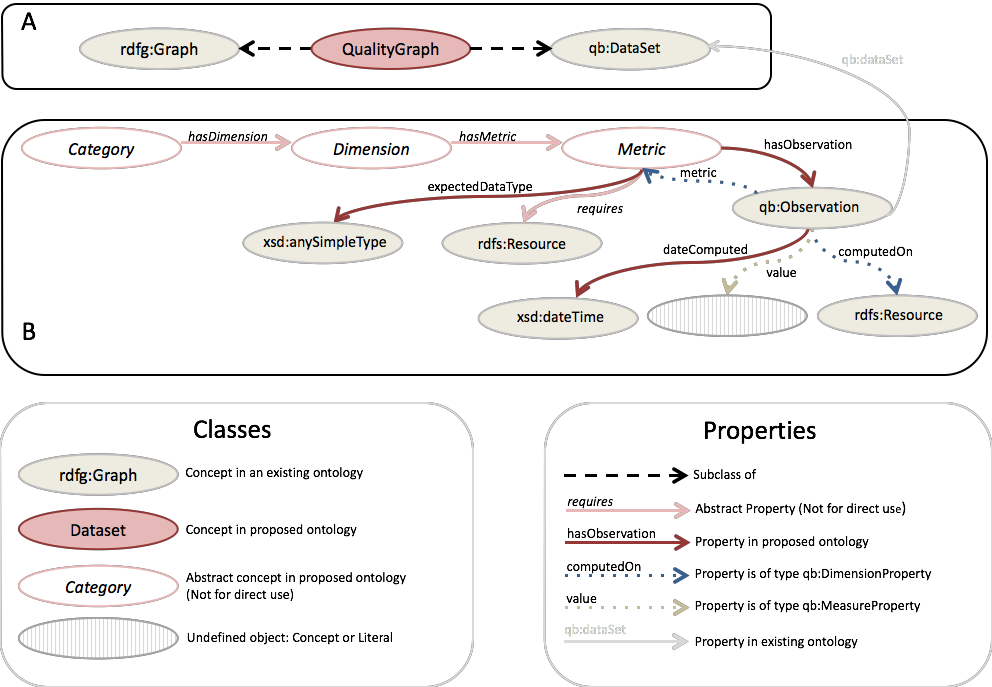
\includegraphics[width=.85\textwidth]{images/daq_extendedframework.png} 
\caption{The extended Dataset Quality Ontology (daQ)}
\label{fig:daqExtended}
\end{figure*}	

Using daQ, the quality metadata is intended to be stored in what we defined to be the \emph{Quality Graph}.
The latter concept is a subclass of \texttt{rdfg:Graph}~\cite{CBHS:NamedGraphs2005}.
This means that the quality metadata \todo{CL@JD: once more I'd rephrase to avoid the impression that \emph{we} are storing stuff.}is stored and managed in a separate named graph from the assessed dataset.
Named graphs are favoured due to
\begin{itemize}
\item the capability of separating the aggregated metadata with regard to computed quality metrics of a dataset from the dataset itself;
\item their use in the Semantic Web Publishing vocabulary~\cite{conf/semweb/CarrollBHS04} to allow named graphs to be digitally signed, thus ensuring trust in the computed metrics and defined named graph instance. Therefore, in principle each \texttt{daq:QualityGraph} can have the following triple \texttt{:myQualityGraph swp:assertedBy :myWarrant .}
\end{itemize}

The daQ ontology distinguishes between three layers of abstraction, based on the survey work by Zaveri et al.~\cite{Zaveri2012:LODQ}.
As shown in Figure~\ref{fig:daqExtended} Box B, a quality graph comprises of a number of different \emph{Categories}, which in turn possess a number of quality \emph{Dimensions}\footnote{In this deliverable we will refer to these as quality dimensions, in order to distinguish between the data cube dimensions}.
A quality dimension groups one or more computed quality \emph{Metrics}.
To formalise this, let $G$ represent the named Quality Graph (\texttt{daq:QualityGraph}), $C = \lbrace c_1, c_2,  \dots , c_x\rbrace$ is the set of all possible quality categories (\texttt{daq:Category}), $D = \lbrace d_1, d_2, \dots , d_y\rbrace$ is the set of all possible quality dimensions (\texttt{daq:Dimension}) and $M = \lbrace m_1, m_2, \dots , m_z\rbrace$ is the set of all possible quality metrics (\texttt{daq:Metric}); where $x,y,z\in \mathbb{N}$, then:

\newtheorem{Def1}{Definition}
\begin{Def1}
\label{def:daq_formalisation}
\begin{align*}
G \subseteq C, \\ 
C \subset D,\\
D \subset M; 
\end{align*}
\end{Def1}

Figure~\ref{fig:venn} shows this formalisation in a pictorial manner using Venn diagrams.

\begin{figure*}[tbph]
\center
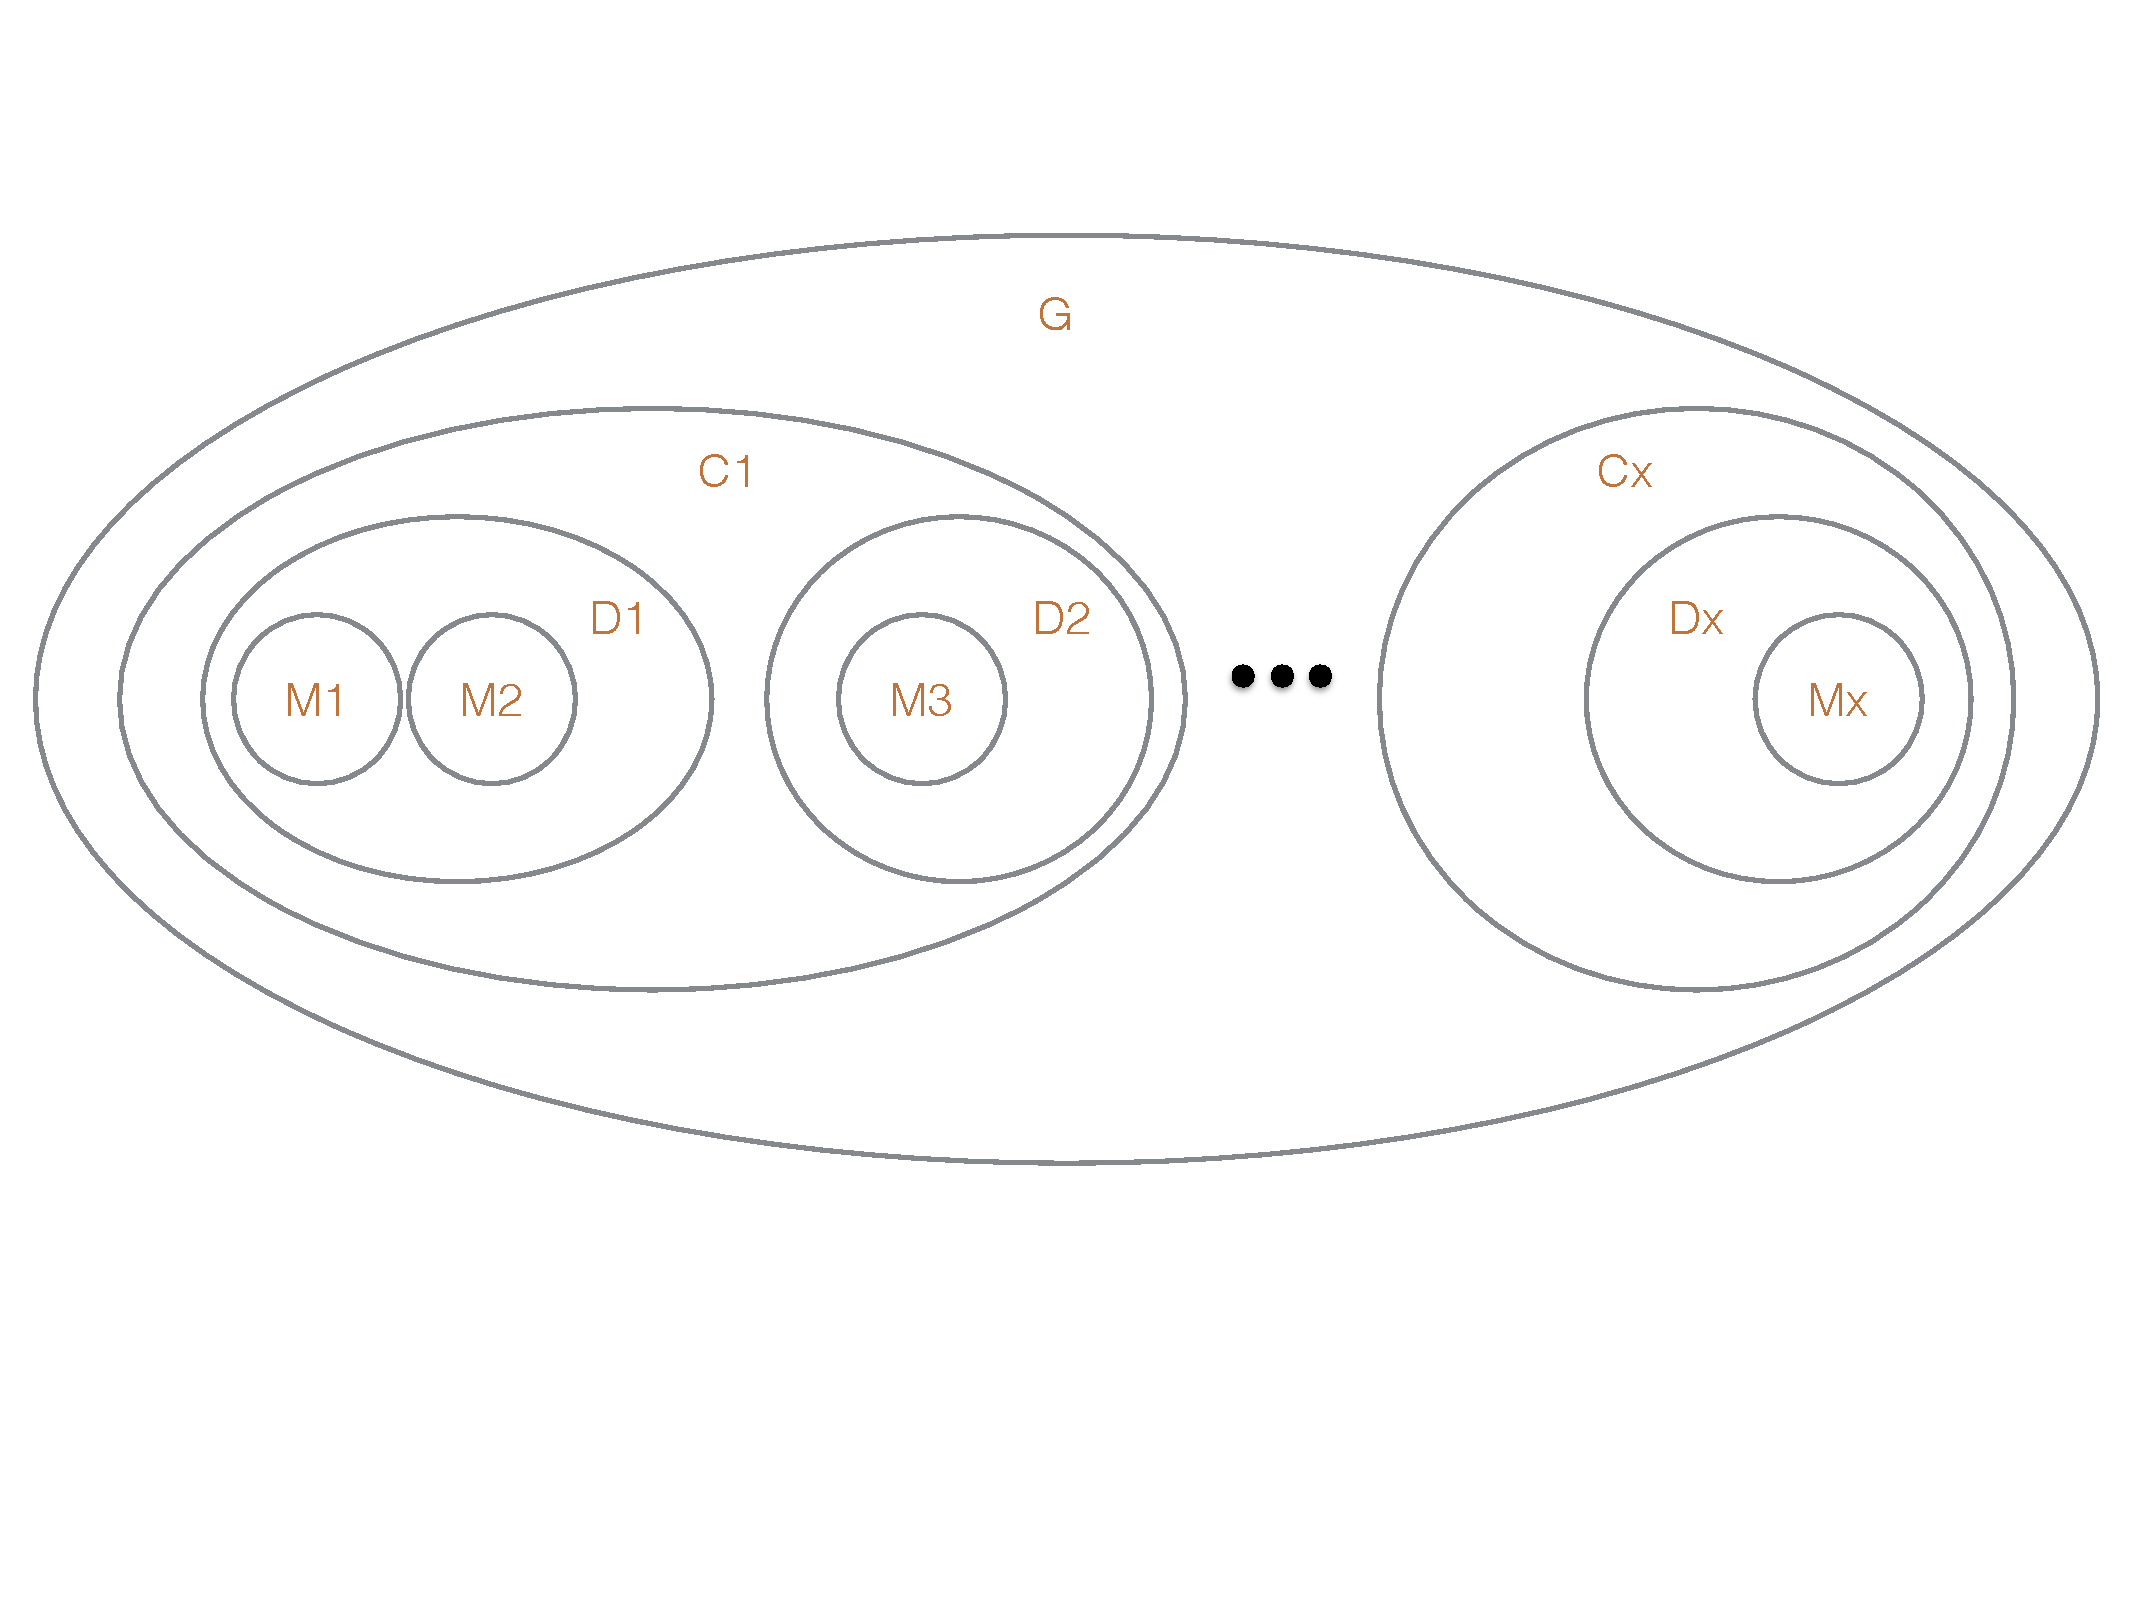
\includegraphics[scale=0.3]{images/venn.pdf} 
\caption{Venn Diagram depicting Definition~\ref{def:daq_formalisation} }
\label{fig:venn}
\end{figure*}

\subsubsection{Extending daQ for Multi-Dimension Representation and Statistical Evaluation}
The Data Cube Vocabulary~\cite{w3c:REC-vocab-data-cube-20140116} allows the representation of statistics about observations in a multidimensional attribute spaces. 
Multidimensional analysis of these observations, e.g.\ across the revision history of a dataset, would thus have required complex querying.
Extending daQ with the standardised Data Cube Vocabulary allows us to represent quality metadata of a dataset as a collection of \emph{Observations}, dimensions being the different quality metrics computed, the resources whose quality is assessed, revisions of these resources, and arbitrary further dimensions, such as the intended application scenario.
It also permits applying the wide range of tools that support data cubes to quality graphs, including the  CubeViz visualisation tool\footnote{\url{http://cubeviz.aksw.org}}.

A \emph{Quality Graph} is a special case of \texttt{qb:DataSet}, which allows us to represent a collection of quality observations complying to  a defined dimensional structure.
Each observation represents a quality metric measured out against a particular resource (e.g.\ a specific revision of a dataset).
daQ defines the structure of such observations by the \texttt{qb:DataStructureDefinition} shown in Listing~\ref{lst:dsd_def}.
\lstinputlisting[caption={The Data Structure Definition (Turtle Syntax)},label=lst:dsd_def, language=N3]{listings/dsd_def.trig}

The \texttt{daq:QualityGraph} also defines one restriction that controls the property \texttt{qb:structure} and its value to the mentioned definition, thus ensuring that all \emph{Quality Graph} instances make use of the standard definition.
Having a standard definition ensures that all \emph{Quality Graph}s conform to a common data structure definition, thus datasets with attached quality metadata can be compared.
Listing~\ref{lst:qg_def} describes the definition of \texttt{daq:QualityGraph}.
\lstinputlisting[caption={The Quality Graph Definition (Turtle Syntax)},label=lst:qg_def, language=N3]{listings/qg_def.trig}

\subsubsection{Abstract Classes and Properties}
This ontology framework (Figure~\ref{fig:daqExtended}) has three abstract classes/concepts (\texttt{daq:Category}, \texttt{daq:Dimension}, \texttt{daq:Metric}) and three abstract properties (\texttt{daq:hasDimension}, \texttt{daq:hasMetric}, \texttt{daq:requires}) which should not be used directly in a quality instance.
Instead these should be inherited as parent classes and properties for more specific quality metrics.
The abstract concepts (and their related properties) are described as follows:

\begin{description}
\item[daq:Category] represents the highest level of quality assessment.
  A category groups a number of dimensions.
\item[daq:Dimension $-$] In each dimension there is a number of metrics.
\item[daq:Metric] is the smallest unit of measuring a quality dimension.
  Each metric instance is linked to one or more observations. 
  Each observation has a value (\texttt{daq:value}), representing a score for the assessment of a quality attribute.
  This attribute is defined as a \texttt{qb:MeasureProperty}.
   Since this value is multi-typed (for example one metric might return true/false whilst another might require a floating point number), the value's \texttt{daq:hasValue} range is inherited by the actual metric's attribute defined by the property \texttt{daq:expectedDataType}.
  An observation must have the Dimension Properties (\texttt{qb:DimensionProperty}) \texttt{daq:computedOn} and \texttt{daq:metric}, which defines the assessed resource and the metric the mentioned resource was assessed by respectively.
  A metric might also require additional information (e.g.\ a gold standard dataset to compare with).
  Therefore, a \todo{CL@JD: to this maybe append ``i.e.\ an instance of a metric class''? - JD: agreed}instance of a metric representation can also define such properties using subproperties of the \texttt{daq:requires} abstract property.
  Another important attribute for any observation is the \todo{CL@JD: do you insist on this custom property, or can't we reuse dcterms:date? - JD: that should be changes, but i'll do it after the deliverable as it will take a lot of effort}\texttt{daq:dateComputed}, where it records the date of the observation's creation.
\end{description}

\subsubsection{Extending daQ for Custom/Specific Quality Metrics}
\label{sec:extendingDAQ}
The classes of the core daQ vocabulary can be extended by more specific and custom quality metrics. 
In order to use the daQ, one should define the quality metrics that characterise the ``fitness for use''~\cite{Juran1974:biblatex} in a particular domain.
We are currently in the process of defining the quality dimensions and metrics described in Deliverable 5.1.
\textbf{Extending} the daQ vocabulary means adding new quality protocols that inherit the abstract concepts (Category-Dimension-Metric).
Custom quality metrics do not need to be included in the daQ namespace itself; in fact, in accordance with LOD best practices, we recommend extenders to make them in their own namespaces.
In Figure~\ref{fig:ext_daq} we show an illustrative example of extending the daQ ontology (TBox) with a more specific quality attribute, i.e.\ the RDF Availability Metric as defined in~\cite{Zaveri2012:LODQ}, and an illustrative instance (ABox) of how it would be represented in a dataset.

The \texttt{Accessibility} concept is defined as an \texttt{rdfs:subClassOf} the abstract \texttt{daq:Category}.
This category has five quality dimensions, one of which is the \textit{Availability} dimension.
This is defined as an \texttt{rdfs:subClassOf} \texttt{daq:Dimension}.
Similarly, \textit{RDFAvailabilityMetric} is defined as an \texttt{rdfs:subClassOf} \texttt{daq:Metric}.
The specific properties \textit{hasAvailabilityDimension} and \textit{hasRDFAccessibilityMetric} (sub-properties of \texttt{daq:hasDimension} and \texttt{daq:hasMetric} respectively) are also defined (Figure~\ref{fig:ext_daq}).

\begin{figure*}[tbph]
\begin{center}
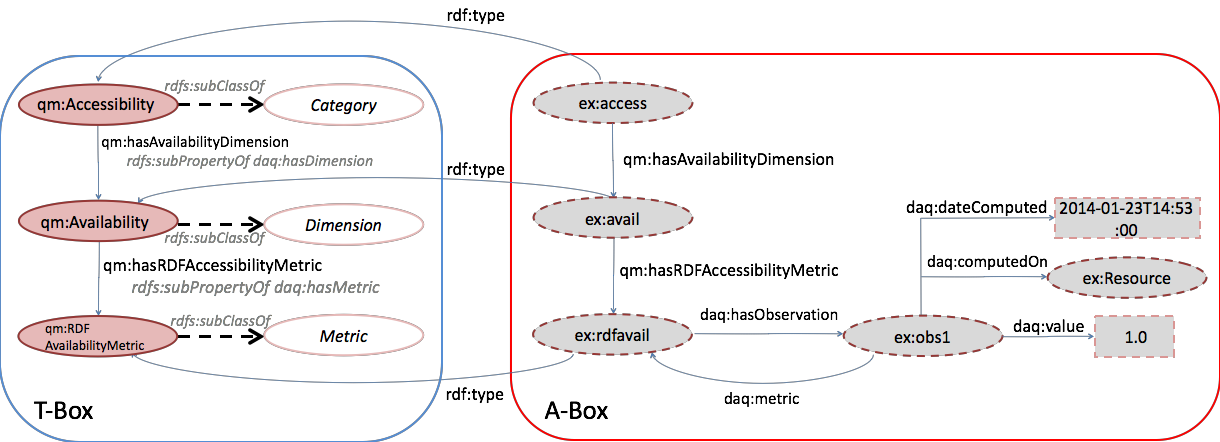
\includegraphics[width=\textwidth]{images/abox-tbox.png}
\caption{Extending the daQ Ontology – TBox and ABox}
\label{fig:ext_daq}
\end{center}
\end{figure*}

\subsubsection{A typical Quality Metadata Graph}
The excerpt listing in~\ref{lst:qg_example} show a typical quality graph metadata in a dataset.
\lstinputlisting[caption={A Quality Graph Excerpt (Turtle Syntax)},label=lst:qg_example, language=N3]{listings/lst1.trig}
The instance \emph{ex:qualityGraph1} is a named \texttt{daq:QualityGraph}.
The defined graph is automatically a \texttt{qb:DataSet}, and due to the restriction placed on the \texttt{daq:QualityGraph} (see Listing~\ref{lst:qg_def}), the value for the \texttt{qb:structure} property is defined as \texttt{daq:dsd} (see Listing~\ref{lst:dsd_def}).
In the named graph, instances for the \texttt{daq:Accessibility}, \texttt{daq:Availability}, \texttt{daq:EndPointAvailabilityMetric} and \texttt{daq:RDFAvailabilityMetric} are shown.
A metric instance has a number of observations.
Each of these observations specifies the metric value (\texttt{daq:value}), the resource the metric was computed on (\texttt{daq:computedOn} – here: different datasets, which are actually different revisions of one dataset), when it was computed (\texttt{daq:dateComputed}), the metric instance (\texttt{daq:metric}) and finally to what dataset the observation is defined in (\texttt{qb:dataSet}).

%%% Local Variables: 
%%% mode: latex
%%% TeX-master: "../../diachron-D5_2"
%%% End: 
